%%%%%%%%%%%%%%%%%%%%%%%%%%%%%%%%%%%%%%%%%
% University of Hong Kong Masters/Doctoral Thesis 
% LaTeX Template
% Version 3.0 (01/07/2020)
% 
% Version 2.x major modifications by:
% Vel (vel@latextemplates.com)
% 
% This template is based on the template by:
% Steve Gunn (http://users.ecs.soton.ac.uk/srg/softwaretools/document/templates/)
% Sunil Patel (http://www.sunilpatel.co.uk/thesis-template/)
% Johannes Böttcher (http://www.latextemplates.com/template/masters-doctoral-thesis)
%
% Template license:
% CC BY-NC-ND 4.0 (https://creativecommons.org/licenses/by-nc-nd/4.0/)
%
% Author:  Nan Meng
% Contact: u3003637@connect.hku.hk
%
%%%%%%%%%%%%%%%%%%%%%%%%%%%%%%%%%%%%%%%%%


%----------------------------------------------------------------------------------------
%	PACKAGES AND OTHER DOCUMENT CONFIGURATIONS
%----------------------------------------------------------------------------------------

\documentclass[
10pt, % The default document font size, options: 10pt, 11pt, 12pt
%oneside, % Two side (alternating margins) for binding by default, uncomment to switch to one side
english, % ngerman for German
onehalfspacing, % Single line spacing (singlespacing), alternatives: onehalfspacing or doublespacing
% draft, % Uncomment to enable draft mode (no pictures, no links, overfull hboxes indicated)
% nolistspacing, % If the document is onehalfspacing or doublespacing, uncomment this to set spacing in lists to single
liststotoc, % Uncomment to add the list of figures/tables/etc to the table of contents
%toctotoc, % Uncomment to add the main table of contents to the table of contents
parskip, % Uncomment to add space between paragraphs
%nohyperref, % Uncomment to not load the hyperref package
headsepline, % Uncomment to get a line under the header
%chapterinoneline, % Uncomment to place the chapter title next to the number on one line
% consistentlayout, % Uncomment to change the layout of the declaration, abstract and acknowledgements pages to match the default layout
]{HKUThesis} % The class file specifying the document structure

\usepackage[utf8]{inputenc} % Required for inputting international characters
\usepackage[T1]{fontenc} % Output font encoding for international characters
\usepackage{fontawesome} % Awesome symbol for usage
\usepackage{wrapfig} % Add enbedded figure in the text
\usepackage{tikz} % Add the signature figure overlap the text
% \usepackage[labelformat=simple]{subcaption} % Add multiple subfigures in a figure environment
% \captionsetup{justification=justified, margin=0pt}
% \renewcommand\thesubfigure{(\Alph{subfigure})} % change the image numbering and reference link to (A),(B),(C), ...... format

\usepackage{mathpazo} % Use the Palatino font by default
% \usepackage[backend=bibtex,style=alphabetic,natbib=true]{biblatex} % Use the bibtex backend with the authoryear citation style (which resembles APA)
\usepackage[natbib=true,maxbibnames=99,firstinits=true]{biblatex}

\addbibresource{thesis.bib} % The filename of the bibliography

\usepackage[autostyle=true]{csquotes} % Required to generate language-dependent quotes in the bibliography

\AtBeginEnvironment{enquote}{\itshape} % change the quote words to italics style

\usepackage{rotating} % Required to add rotated big tables

\usepackage[normalem]{ulem} % Required to add dashed underlines

\setlength\parindent{2em}
%----------------------------------------------------------------------------------------
%	MARGIN SETTINGS
%----------------------------------------------------------------------------------------

\geometry{
	paper=a4paper, % Change to letterpaper for US letter
	left=3.5cm, % Left margin
	right=3.6cm, % Right margin
	bindingoffset=.5cm, % Binding offset
	top=2.5cm, % Top margin
	bottom=2.5cm, % Bottom margin
	%showframe, % Uncomment to show how the type block is set on the page
}


%----------------------------------------------------------------------------------------
%	THESIS INFORMATION
%----------------------------------------------------------------------------------------

\thesistitle{HKU Doctoral Thesis Template}
% Thesis title, this is used in the title and abstract, print it elsewhere with \ttitle

\supervisor{Prof. FirstName \textsc{FamilyName}}
% Your supervisor's name, this is used in the title page, print it elsewhere with \supname

\cosupervisor{Prof. FirstName \textsc{FamilyName}}
% Your supervisor's name, this is used in the title page, print it elsewhere with \supname
% \cosupervisor{Prof. Hayden K.-H. \textsc{So}} % Your supervisor's name, this is used in the title page, print it elsewhere with \cosupname

\examiner{}
% Your examiner's name, this is not currently used anywhere in the template, print it elsewhere with \examname

\degree{Doctor of Philosophy}
% Your degree name, this is used in the title page and abstract, print it elsewhere with \degreename

\author{FirstName \textsc{FamilyName}}
% The author name, this is used in the title page and abstract, print it elsewhere with \authorname

\addresses{}
% Your address, this is not currently used anywhere in the template, print it elsewhere with \addressname

\subject{Computer Vision}
% Your subject area, this is not currently used anywhere in the template, print it elsewhere with \subjectname

\keywords{Light field, high-dimensional convolutional neural network, deep learning}
% Keywords for your thesis, this is not currently used anywhere in the template, print it elsewhere with \keywordnames

\university{University of Hong Kong}
% Your University's name and URL, this is used in the cover page and abstract, print it elsewhere with \univname

\bsuniversity{HKU}
\msuniversity{HKU}
% Your Bachelor/Master University's name and URL, this is used in the title page and abstract, print it elsewhere with \univname

\department{Department Name}
% Your department's name and URL, this is used in the title page and abstract, print it elsewhere with \deptname

\group{Laboratory of The Student}
% Your research group's name and URL, this is used in the title page, print it elsewhere with \groupname

\faculty{Faculty Name}
% Your faculty's name and URL, this is used in the title page and abstract, print it elsewhere with \facname

\AtBeginDocument{
\hypersetup{pdftitle=\ttitle} % Set the PDF's title to your title
\hypersetup{pdfauthor=\authorname} % Set the PDF's author to your name
\hypersetup{pdfkeywords=\keywordnames} % Set the PDF's keywords to your keywords
}
% \AtBeginEnvironment{algorithm}{\setstretch{2}}
\setlength{\algomargin}{1.3ex}


%----------------------------------------------------------------------------------------
%	NEW COMMAND DEFINITION
%----------------------------------------------------------------------------------------
\newcommand{\codestyle}[1]{\colorbox{gray!20}{\darkred{#1}}}

% ======================================================================================== %
%                                        START DOCUMENT
% ======================================================================================== %

\begin{document}

\frontmatter % Use roman page numbering style (i, ii, iii, iv...) for the pre-content pages
\pagestyle{plain} % Default to the plain heading style until the thesis style is called for the body content


%----------------------------------------------------------------------------------------
%	COVER
%----------------------------------------------------------------------------------------

\begin{titlepage}
\addtocounter{page}{-1}
\begin{center}

% \vspace*{.024\textheight}
\begin{tabular}{cc}
    
\includegraphics[align=c, width=0.18\textwidth]{Covers/hkulogo.png} &  
    {\scshape \huge \darkred{\univname}} % University name
\end{tabular}

\vspace{0.5cm}
\textsc{\Large Doctoral Thesis}\\[0.5cm] % Thesis type


\rule[0.4cm]{13cm}{0.1pt}\\% \HRule \\[0.4cm] % Horizontal line
{\huge \bfseries \ttitle\par}\vspace{0.4cm} % Thesis title
% \HRule \\[1.5cm] % Horizontal line
\rule{13cm}{0.1pt}\\ \vspace{1.5cm}
 
\begin{minipage}[t]{0.4\textwidth}
\begin{flushleft} \large
\emph{Author:}\\
\href{http://#}{\authorname} % Author name - remove the \href bracket to remove the link
\end{flushleft}
\end{minipage}
\begin{minipage}[t]{0.4\textwidth}
\begin{flushright} \large
\emph{Supervisor:} \\
\href{https://www.eee.hku.hk/~elam/}{\supname} \\ % Supervisor name - remove the \href bracket to remove the link
\emph{Co-Supervisor:} \\
\href{https://www.eee.hku.hk/~hso/}{\cosupname} % Supervisor name - remove the \href bracket to remove the link 
\end{flushright}
\end{minipage}\\[1.6cm]
 
\vfill

\large \textit{A thesis submitted in fulfillment of the requirements\\ for the degree of \degreename}\\[0.3cm] % University requirement text
\textit{in the}\\[0.4cm]
% \groupname\\
\deptname\\\facname\\[1.6cm] % Research group name and department name
 
\vfill

{\large \usdate\today}\\[4cm] % Date
%\includegraphics{Logo} % University/department logo - uncomment to place it
 
\vfill
\end{center}

\end{titlepage}


\blankpage
\addtocounter{page}{-1}


%----------------------------------------------------------------------------------------
%	ABSTRACT PAGE
%----------------------------------------------------------------------------------------


\begin{abstract}
\addchaptertocentry{\abstractname} % Add the abstract to the table of contents
Put Your \emph{Abstract} Here ...

\bigskip
\noindent This latex project is a doctoral thesis template for the University of Hong Kong. The style and design of the entire project closely follow the official guidelines from the Graduate School: \href{https://intraweb.hku.hk/reserved_1/gradsch/PreparingandSubmittingYourThesis.pdf}{\textbf{Preparing and Submitting Your Thesis --- A Guide for MPhil and PhD Students.}} Generally, there is no strict stipulations on the style or format of different components of the thesis, except for the \textbf{Abstract}. According to the detailed regulations [\href{https://intraweb.hku.hk/reserved_1/gradsch/regulations_procedures/format_binding_presentation.pdf}{\textbf{Link}}], the \textbf{Abstract} should be part of the thesis with \uline{no fewer than 200 and no more than 500 words}. The format shall be the same as that of the thesis itself. The front page of each abstract shall contain the statement which includes:
\begin{itemize}
    \item Abstract of thesis entitled ``\dotuline{\hspace{8cm}}''
    \item Submitted by \dotuline{\hspace{10cm}}~
    \item for the degree of \dotuline{\hspace{9.5cm}}~
    \item at the \univname~in (\usdate\today).
\end{itemize}

In addition to the opening of abstract, the abstract \uline{should appear before the title page}. The abstract in this template is \uline{not numbered, or counted in the pagination of the front matter, or listed in the table of contents}. All the requirements are fulfilled in this template.


\bigskip
\noindent \textbf{\Large How to adjust the typeset of Abstract}

\noindent The typeset of the opening of abstract page is defined in the class file \codestyle{HKUThesis.cls} \textbf{Line 507-529}. Users can adjust the typeset by changing the settings. The layout of the main text is consistent with other parts of the thesis.


\bigskip

\noindent \textbf{Note that:} Considering the university may change its standards over time, users are not supposed to 100 percent ``trust'' this template. Even though the template is prepared strictly follow the stipulations of the Graduate School of The University of Hong Kong, this is \textbf{not an official} template and we are \textbf{not responsible} for any problems of your thesis submission caused by the format, style, typeset, etc of the template. We \textbf{strongly suggest} the users to read the latest \href{https://www.gradsch.hku.hk/gradsch/current-students/thesis-submission/guidelines-on-thesis-submission}{\textbf{Guidelines on Thesis Submission}} carefully and adjust the template accordingly to satisfy the stipulations of the university.

\end{abstract}


%----------------------------------------------------------------------------------------
%	TITLE PAGE
%----------------------------------------------------------------------------------------
\pagestyle{empty}
\newpage
\addtocounter{page}{-1}
\begin{center}
\vspace*{2cm}
\huge{ \bf \ttitle}
\end{center}

\vspace{20mm}
\begin{center}
by

\vspace{10mm}
{\bf \authorname}\\
B.S. \textit{\bsunivname} M.S. \textit{\msunivname}
\end{center}

\vspace{30mm}
\begin{center}
A Thesis Submitted in Partial Fulfilment \\
of the Requirements for the Degree of \\
Doctor of Philosophy \\
\vspace{10mm}
at \\
\vspace{10mm}
\univname\\
%February 2015
\monthyeardate\today
\end{center}

%----------------------------------------------------------------------------------------
%	COPYRIGHT PAGE
%----------------------------------------------------------------------------------------

\newpage
\thispagestyle{empty}
\addtocounter{page}{-1}
\vspace*{\fill}
\scshape \noindent Copyright \copyright 2020, by \authorname \\
\noindent all rights reserved.
\vspace*{\fill}
\newpage
\rm


%----------------------------------------------------------------------------------------
%	DECLARATION PAGE
%----------------------------------------------------------------------------------------

\begin{declaration}
\setcounter{page}{1}
\addchaptertocentry{\authorshipname} % Add the declaration to the table of contents

\vspace{0.6cm}
I, \authorname, declare that this thesis titled, \enquote{\ttitle}, which is submitted in fulfillment of the requirements for the Degree of Doctor of Philosophy, represents my own work except where due acknowledgement have been made. I further declared that it has not been previously included in a thesis, dissertation, or report submitted to this University or to any other institution for a degree, diploma or other qualifications.


\vspace{2cm} 
\begin{flushright}
\hfill Signed: \underline{\hspace{5cm}}\\[2em] % This prints a line for the signature
\hfill Date: \underline{\hspace{1.5cm} \usdate\today \hspace{1.5cm}}\\ % This prints a line to write the date
\end{flushright}

% Signature
\begin{tikzpicture}[remember picture,overlay]
\node[xshift=-6cm,yshift=-18cm] at (current page.north east){%
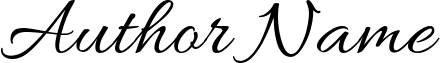
\includegraphics[width=3.6cm]{Figures/signature.png}};
\end{tikzpicture}
\end{declaration}





%----------------------------------------------------------------------------------------
%	QUOTATION PAGE
%----------------------------------------------------------------------------------------

\newpage
\thispagestyle{empty}
\vspace*{\fill}
\begin{center}
% Font family: ''Calling Angels Personal Use'' from website https://www.dafont.com

\includegraphics[width=0.8\textwidth]{Dedication/dedication.pdf}
\end{center}
\vspace*{\fill}



%----------------------------------------------------------------------------------------
%	ACKNOWLEDGEMENTS
%----------------------------------------------------------------------------------------
\begin{acknowledgements}
\setcounter{page}{2}
\addchaptertocentry{\acknowledgementname} % Add the acknowledgements to the table of contents
\vspace{1cm}


\noindent I would like to thank...
\\[0.4cm]

% \hfill
\begin{flushright}
    \authorname \\
    University of Hong Kong \\
    \usdate\today
\end{flushright}

\end{acknowledgements}

%----------------------------------------------------------------------------------------
%	LIST OF PUBLICATIONS PAGES
%----------------------------------------------------------------------------------------
\begin{publications}
\addcontentsline{toc}{chapter}{List of Publications}
\newcommand{\JourConfTitle}[1]{\ul{\emph{#1}}}

% ---------------------------------------------------------------------------
% JOURNALS
% ---------------------------------------------------------------------------

\begin{journals}
\item \textbf{Nan Meng}, Hayden K.-H. So, Xing Sun, and Edmund Y. Lam, ``High-dimens-ional dense residual convolutional neural network for light field reconstruction,'' \JourConfTitle{IEEE Transactions on Pattern Analysis and Machine Intelligence}, October 2019.

\item \textbf{Nan Meng}, Zhou Ge, Tianjiao Zeng, and Edmund Y. Lam, ``LightGAN: a deep generative model for light field reconstruction,'' \JourConfTitle{IEEE Access}, June 2020.

\item \textbf{Nan Meng}, Xing Sun, Hayden K.-H. So, and Edmund Y. Lam, ``Computational light field generation using deep nonparametric Bayesian learning,'' \JourConfTitle{IEEE Access}, vol. 7, pp. 24990--25000, February 2019.

\item \textbf{Nan Meng}, Edmund Y. Lam, Kevin K.-M. Tsia and Hayden K.-H. So, ``Large-scale multi-class image-based cell classification with deep learning,'' \JourConfTitle{IEEE Journal of Biomedical and Health Informatics}, vol. 23, no. 5, pp. 2091--2098, September 2019. 
\end{journals}

% \newpage
% ---------------------------------------------------------------------------
%  CONFERENCES
% ---------------------------------------------------------------------------

\begin{conferences}
\item \textbf{Nan Meng}, Xiaofei Wu, Jianzhuang Liu, and Edmund Y. Lam, ``High-order residual network for light field super-resolution,'' in \JourConfTitle{Association for the Advancement of Artificial Intelligence}, vol. 34, no.7, pp. 11757-11764, 2020.

\item \textbf{Nan Meng}, Tianjiao Zeng, and Edmund Y. Lam, ``Spatial and angular reconstruction of light field based on deep generative networks,'' in \JourConfTitle{IEEE International Conference on Image Processing}, pp. 4659–4663, September 2019.

\item \textbf{Nan Meng}, Tianjiao Zeng, and Edmund Y. Lam, ``Perceptual loss for light field reconstruction in high-dimensional convolutional neural networks,'' in \JourConfTitle{OSA Topical Meeting in Computational Optical Sensing and Imaging}, pp. CW1A.5, June 2019.

\item Edmund Y. Lam, \textbf{Nan Meng}, and Hayden K.H. So, ``Deep convolutional neural network for single-cell image analysis,'' in \JourConfTitle{High-Speed Biomedical Imaging and Spectroscopy: Toward Big Data Instrumentation and Management}, volume 10505 of Proceedings of the SPIE, pp. 105050K, January 2018.

\item \textbf{Nan Meng}, Hayden K.-H. So, and Edmund Y. Lam, ``Computational single-cell classification using deep learning on bright-field and phase images,'' in \JourConfTitle{IAPR Conference on Machine Vision Applications}, pp. 164–167, May 2017.

\item Xing Sun, Zhimin Xu, \textbf{Nan Meng}, Edmund Y. Lam, and Hayden K.-H. So, ``Data-driven light field depth estimation using deep convolutional neural networks,'' in \JourConfTitle{IEEE International Joint Conference on Neural Networks}, pp. 367–374, July 2016.

\item Xing Sun, \textbf{Nan Meng}, Zhimin Xu, Edmund Y. Lam, and Hayden K.-H. So, ``Sparse hierarchical nonparametric Bayesian learning for light field representation and denoising,'' in \JourConfTitle{IEEE International Joint Conference on Neural Networks}, pp. 3272–3279, July 2016.
\end{conferences}

\begin{patents}
\item \textbf{Nan Meng}, Xiaofei Wu, Jianzhuang Liu, ``Image Enhancement and Reconstruction based on Camera Array'', [\emph{under review}]
\end{patents}

\begin{datasets}
\item \textbf{Nan Meng}, Edmund Lam, Tsia, Kevin Kin Man, So, Hayden Kwok-Hay, ``Human somatic label-free bright-field cell images'', IEEE Dataport, 2018. [\darkred{Online}]. Available: \url{http://dx.doi.org/10.21227/H2QW97}. Accessed: Mar. 13, 2019.
\end{datasets}

\end{publications}


%----------------------------------------------------------------------------------------
%	LIST OF CONTENTS/FIGURES/TABLES PAGES
%----------------------------------------------------------------------------------------

\tableofcontents % Prints the main table of contents

\listoffigures % Prints the list of figures

\listoftables % Prints the list of tables

\listofalgorithms % Prints the list of algorithms
\addchaptertocentry{\listalgorithmcfname}
%----------------------------------------------------------------------------------------
%	ABBREVIATIONS
%----------------------------------------------------------------------------------------
\begin{abbreviations}{ll} % Include a list of abbreviations (a table of two columns)

\textbf{ASAP} & \textbf{A}s \textbf{S}oon \textbf{A}s \textbf{P}ossible \\
\textbf{AKA} & \textbf{A}lso \textbf{K}nown \textbf{A}s \\
\textbf{BPFA} & \textbf{B}eta \textbf{P}rocess \textbf{F}actor \textbf{A}nalysis \\
\textbf{CNN} & \textbf{C}onvolutional \textbf{N}eural \textbf{N}etwork \\
\textbf{GAN} & \textbf{G}enerative \textbf{A}dversarial \textbf{N}etwork \\
\textbf{MSE} & \textbf{M}ean \textbf{S}quare \textbf{E}rror \\
\textbf{PSNR} & \textbf{P}eak \textbf{S}ignal-to-\textbf{N}oise \textbf{R}atio \\
\textbf{SSIM} & \textbf{S}tructural \textbf{SIM}ilarity \\

\end{abbreviations}


%----------------------------------------------------------------------------------------
%	SYMBOLS
%----------------------------------------------------------------------------------------
\begin{symbols}{p{0.15\textwidth}p{0.7\textwidth}l} % Include a list of Symbols (a three column table)

\multicolumn{3}{l}{\symboltitle{Global notations}}\\ \\
$I^\mathrm{SR}$ & super-resolved light field image & --- \\
$I^\mathrm{LR}$ & low-resolution light field image & --- \\
$I^\mathrm{HR}$ & high-resolution light field image & --- \\
$E^\mathrm{SR}$ & super-resolved epipolar plane image & --- \\
$E^\mathrm{HR}$ & high-resolution epipolar plane image & --- \\ \\
% $L$ & light field function & --- \\

\multicolumn{3}{l}{\symboltitle{Chapter~1}}\\ \\
$\theta$, $\phi$ & incoming direction expressed in term of spherical coordinates & rad \\
$\tau$ & time & s (second)\\
$x$,$y$ & spatial coordinates with two-plane parameterization & 1 (uint) \\
$s$,$t$ & angular coordinates with two-plane parameterization & 1 (uint) \\
$P$ & radiance distribution & \si{\watt\per\steradian \square{\metre} \text{\hertz}} \\
$\Omega$ & image plane & --- \\
$\Theta$ & parameters of the multi-layer framework & --- \\
$\gamma_s$, $\gamma_a$ & scaling factors of spatial / angular coordinates & 1 (uint) \\
$\mathcal{L}$ & loss function & --- \\ \\

\multicolumn{3}{l}{\symboltitle{Chapter~2}}\\ \\
$F_0$ & shallow features extracted by a single HConv layer & --- \\
$F_\mathrm{G_d}$ & feature maps extracted by the $d^\mathrm{th}$ HRB of the GRLNet & --- \\
$H_\mathrm{HRB}^\mathrm{n}$ & the operation of the $n^\mathrm{th}$ HRB of the SReNet & --- \\
$H_\mathrm{AGBN}$ & the operation of the proposed aperture group batch normalization algorithm & --- \\
$H_\mathrm{up}$ & upsampling operation on the low-resolution features & --- \\ \\


$\ell_A$ & angular loss & --- \\
$\ell_S$ & spatial perceptual loss & --- \\ 
$\ell_{SA}$ & the weighted combination of $\ell_A$ and $\ell_S$& --- \\
$f$ & the summation of all the feature maps after every activation function of VGG network & --- \\
$g$ & learned mapping between the low-resolution and high-resolution light field images & --- \\ \\


\multicolumn{3}{l}{\symboltitle{Chapter~3}}\\ \\
$x$,$y$ & spatial coordinates with two-plane parameterization & 1 (uint) \\
$s$,$t$ & angular coordinates with two-plane parameterization & 1 (uint) \\
$\gamma_s$, $\gamma_a$ & scaling factors of spatial / angular coordinates & 1 (uint) \\
$\ell_G$ & generator adversarial loss & --- \\
$\phi$ & denotes the mapping of VGG network & --- \\
$\delta$ & nearest neighbor downsampling operator & --- \\
$\kappa$ & a Gaussian blurring kernel with a window size of $7 \times 7$ and standard deviation of 1.2 pixels & --- \\
$\eta$ & additive noise with zero mean and unit standard deviation & --- \\ \\

\end{symbols}


%----------------------------------------------------------------------------------------
%	THESIS CONTENT - CHAPTERS
%----------------------------------------------------------------------------------------

\mainmatter % Begin numeric (1,2,3...) page numbering

\pagestyle{thesis} % Return the page headers back to the "thesis" style

% Include the chapters of the thesis as separate files from the Chapters folder
% Uncomment the lines as you write the chapters

% Chapter 1

\chapter{Introduction} % Main chapter title

\label{Chapter1} % For referencing the chapter elsewhere, use \ref{Chapter1} 

%----------------------------------------------------------------------------------------

% Define some commands to keep the formatting separated from the content 
% \newcommand{\keyword}[1]{\textbf{#1}}
% \newcommand{\tabhead}[1]{\textbf{#1}}
% \newcommand{\code}[1]{\texttt{#1}}
% \newcommand{\file}[1]{\texttt{\bfseries#1}}
% \newcommand{\option}[1]{\texttt{\itshape#1}}

%----------------------------------------------------------------------------------------

% =========================================================== %
%                 Section: General Information                %
% =========================================================== %
\section{General Information}
\label{chap1:sec1:general_information}
This template is for MPhill/Doctor students of University of Hong Kong to prepare their theses. The entire project strictly follows the requirements of \uline{booklet provided by Graduate School of the University of Hong Kong}. The current version of this template is prepared according to the $\boldsymbol{13^\mathrm{th}}$ edition of the booklet entitled ``\href{https://intraweb.hku.hk/reserved_1/gradsch/PreparingandSubmittingYourThesis.pdf}{Preparing and Submitting Your Thesis --- A Guide for MPhil and PhD Students.}'' This edition is updated in \textbf{July 2019}. Considering the university may change the stipulations over time, this template also provides the guidelines to adjust the typeset. The current version of the template has been tested by the author(s) and has been successfully accepted by the Engineering Faculty.
However, \uline{users should also notice that this is not an official template, and we are not responsible for any problems of your thesis preparation and submission caused by using this template.} For anyone who would like to use this template, you have to be responsible for your thesis and your are supposed to carefully read and follow the rules in the latest edition of the university booklet to prepare your thesis. In the rest of the template, we will demonstrate how to use, change, or adjust this template.


% =========================================================== %
%      Section: General Requirements of Graduate School       %
% =========================================================== %
\section{General Requirements of Graduate School}
\label{chap1:sec2:general_requirements_of_graduate_school}
According to the \href{https://intraweb.hku.hk/reserved_1/gradsch/PreparingandSubmittingYourThesis.pdf}{$13^\mathrm{th}$ edition booklet}, ``The Thesis Format'' section, the thesis submitted for examination shall be typewritten or printed on one side or both sides of International size A4 paper, with a margin of not less than 35mm on both right and left-hand edges of each page (as shown in \figref{fig:chap1:thesis_requirements}).
\begin{figure}[!h]
    \centering
    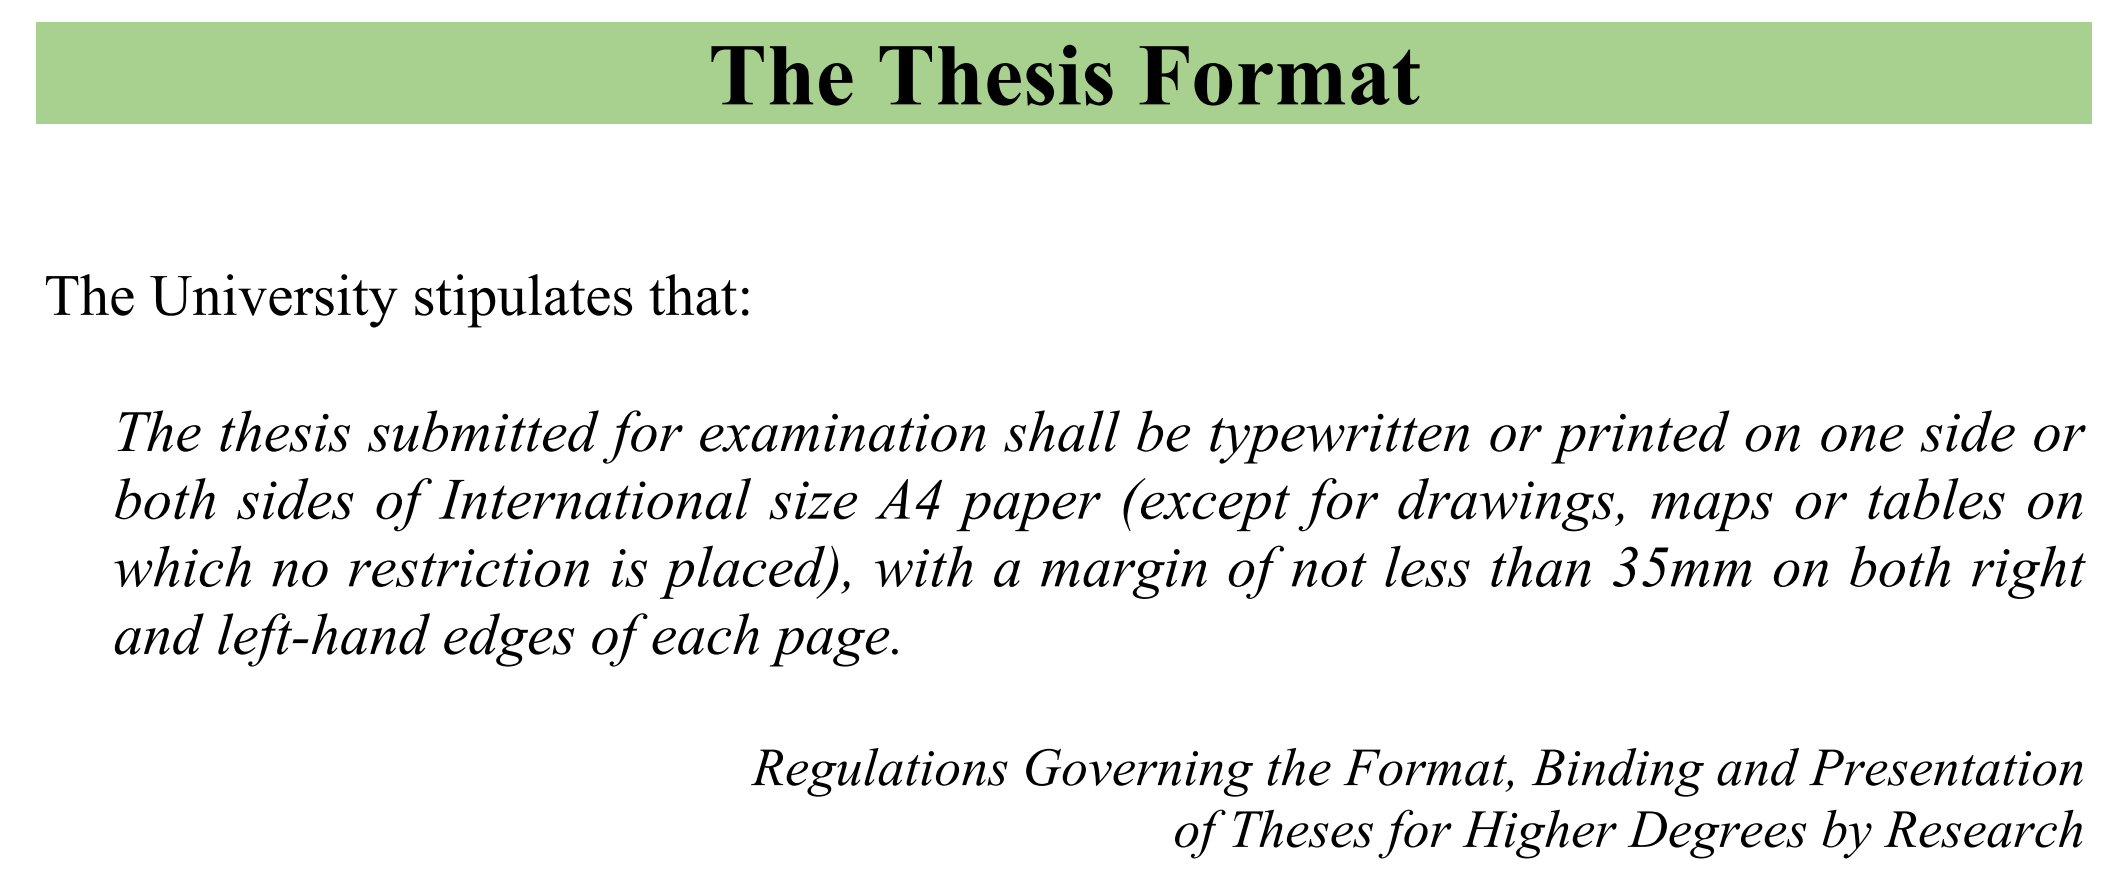
\includegraphics[width=.96\textwidth]{Figures/Chapter1/thesis_requirement.PNG}
    \caption{Requirements of the thesis format in the Graduate School $13^\mathrm{th}$ edition booklet at Page 9.}
    \label{fig:chap1:thesis_requirements}
\end{figure}


% =========================================================== %
%                    Subsection: Page Margin                  %
% =========================================================== %
\subsection{Page Margin}
\label{chap1:sec:2:subsec1:page_margin}
The format of page size and margin is defined in ``main.tex'' file \textbf{Line 63-71}. The page margin of the current version template is \uline{Left: 35mm, Right: 36mm (a4paper).} Users can change the page margin by adjusting the corresponding settings. There is no stipulation for the top and bottom margins, but the booklet recommend that both of them should be 25mm, which is adopted in this template. 


% =========================================================== %
%          Subsection: Font, Alignment, Line Spacing          %
% =========================================================== %
\subsection{Font, Alignment, Line Spacing}
Ordinarily, there is no restrict stipulation for the font family, font size, alignment, and line spacing. All of these are a matter of personal preference. This template uses \textit{10pt} font size, \textit{Fully Justified} alignment style and \textit{One and A Half} line spacing. Users can adjust the settings in \textbf{Line 19-33} of the ``main.tex'' file to change the typeset.


% =========================================================== %
%                      Subsection: Contents                   %
% =========================================================== %
\subsection{Contents}
The contents of this template can be subdivided into three parts --- the front matter, the text and the back matter, which strictly follows the stipulations of the official booklet (Page 17). \tabref{chap1:longtable:checking_list} indicates the what contents are required in the submitted thesis and what contents are optional. The column ``Required'' denotes that 
\begin{center}
\begin{longtable}{|l|c|c|}
\caption{Checking list indicating the contents should be included in the thesis.}\label{chap1:longtable:checking_list}\\
\hline
\textbf{The Front Matter} & Required     &  Include $\checkmark$ \\ \hline \hline
Abstract                  & Yes          & $\checkmark$         \\
Title Page                & Yes          & $\checkmark$         \\
Frontispiece              &              &                      \\
Dedication                &              & $\checkmark$         \\
Epigraph                  &              &                      \\
Declarations              & Yes          & $\checkmark$         \\
Acknowledgements          &              & $\checkmark$         \\
Table of Contents         & Yes          & $\checkmark$         \\
List of Illustrations     &              &                      \\
List of Figures           &              & $\checkmark$         \\
List of Tables            &              & $\checkmark$         \\
List of Algorithm         &              & $\checkmark$         \\
List of Abbreviations     &              & $\checkmark$         \\
List of Symbols           &              & $\checkmark$         \\
Others                    &              &                      \\ \hline \hline
\textbf{The Text}         & Yes          & $\checkmark$         \\ \hline \hline
\textbf{The Reference or Back Matter} &    ---    &   ---       \\ \hline \hline
Glossary                  &              &                      \\
Appendices                &              &                      \\
Notes                     &              &                      \\
Bibliography or Reference List & Yes          &  $\checkmark$   \\
Index                     &              &                      \\
\hline
\end{longtable}
\end{center}
This template support most of the contents listed in the figure, including the ``Abstract'', ``Title Page'', ``Declarations'', ``Acknowledgements'', ``List of Publications'', ``Contents'', ``List of Figures'', ``List of Tables'', ``List of Algorithms'', ``List of Abbreviations'', ``List of Symbols'', ``Main Text'', ``Appendices'', and ``Bibliography''. Each part is defined in an independent tex file and the ``main.tex'' file combines all the different parts to form the entire thesis. Therefore, users can easily make the changes by adjusting the corresponding document files.

In addition to the stipulations of the booklet, this template also provides a beautiful \textbf{cover page}, which is the first two pages of this project. \uline{The cover page is \textbf{not required} by the Graduate School and you'd better remove the cover page when bounding your thesis for submission.}









% Chapter 2

\chapter{Guidelines on Adjustments} % Main chapter title

\label{Chapter2} % For referencing the chapter elsewhere, use \ref{Chapter2} 

%----------------------------------------------------------------------------------------

% Define some commands to keep the formatting separated from the content 
% \newcommand{\keyword}[1]{\textbf{#1}}

%----------------------------------------------------------------------------------------
This chapter demonstrates how to make changes and DIY the thesis style when using this template. For each component of the thesis, we provide both 

\section{Title Page}
\textbf{Title Page} is designed to obviously bear the title of the thesis and the author's name. Users can add any degrees or professional qualifications that he/she holds as well as the author's name in the national script. Both the title and the author's name are highlighted in blod style. Given that there may also be an oral and/or written examination, and thus this template uses the following form of words:

\begin{quote}
A thesis submitted in partial fulfilment of the requirements for the degree of Doctor (or Master) of Philosophy at The University of Hong Kong.
\end{quote}

\noindent The title page is not numbered, or counted in the pagination of the front mater, or listed in the table of contents. The document for title page is quite simple, which can be found in the path \colorbox{gray!20}{Titlepage/titlepage.tex}.


\section{Dedication}
\label{chap2:sec2:dedication}
\textbf{Dedication} is a place to show your wish to dedicate the thesis to friends, family or loved ones. This template uses a single page example for dedication, as shown in \figref{fig:chap2:dedication_sample}. This page is not numbered, or counted in the pagination of the front matter, or listed in the table of contents.
\begin{figure}
    \centering
    
\includegraphics[width=.6\textwidth]{Dedication/dedication.pdf}
    \caption{An example dedication page.}
    \label{fig:chap2:dedication_sample}
\end{figure}


\section{Epigraph}
\label{chap2:sec3:epigraph}
\textbf{Epigraph} is a relevant quotation on the subject of the thesis, or some general guidelines or philosophical principles. Ordinarily, the author and source of the quotation should also be given. This page is not included in the template and users can add the epigraph page according to their willingness.


\section{Declarations}
\label{chap2:sec4:declarations}
\textbf{Declarations} page is a required item according to the official booklet. The contents of declaration are in terms of the official sample (\textit{Sample Page 6} on page 41 of the booklet) with some minor changes to specify the author's name and thesis title.


\section{Acknowledgements}
\label{chap2:sec5:acknowledgements}
\textbf{Acknowledgements} is the place where the author thanks mentors, labmates, colleagues, friends, family members and also the financial support from scholarships and research grants. Each page of the acknowledgements is numbered in lower case Roman numerals


\section{Table of Contents}
\label{chap2:sec6:table_of_contents}
\textbf{Table of Contents} in this template is simply headed ``Contents'' which lists all the parts of the thesis and the page on which they commence. Each of the chapters, sections and subsections are included in the list. The capitalization and wording of the titles listed in the table exactly agree with the corresponding ones appear in the body text. If users would like to include some optional pages in the Table of Contents, such as the Frontispiece page or Epigraph page, they can simply add a command \verb|\addchaptertocentry{\pagename}| at the corresponding page. For example, your can add the \textit{Abstract} item to the Table of Contents, by adding the command to the file \codestyle{Abstract/abstract.tex}, as shown in \figref{fig:chap2:example_add_command}.
\begin{figure}[!h]
    \centering
    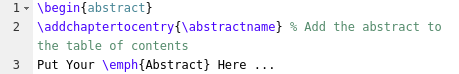
\includegraphics[width=.8\textwidth]{Figures/Chapter2/add_command_example.png}
    \caption{An example of how to add chapter to the Table of Contents.}\label{fig:chap2:example_add_command}
\end{figure}


\section{List of Tables, Figures and Algorithms, etc}
\label{chap2:sec7:list_of_tables_figures_and_algorithms_etc}
\begin{figure}[t]
    \centering
    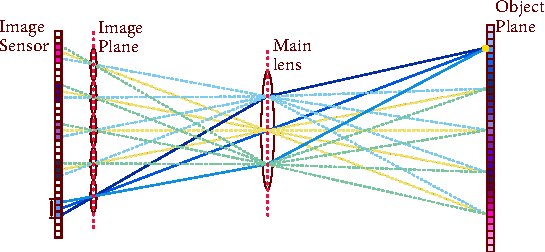
\includegraphics[width=0.6\textwidth]{Figures/Chapter2/photo_consistency.pdf}
    \caption{Light transformation model in a plenoptic camera. Within a plenoptic camera, a micro-lens array has been placed at the image plane, which further splits the incoming light rays from different directions and records them separately. Therefore, the multi-view information can be extracted from each light field image captured by a single shot.}
    \label{fig:photo_consistency}
\end{figure}

\begin{figure}[t]
    \centering
    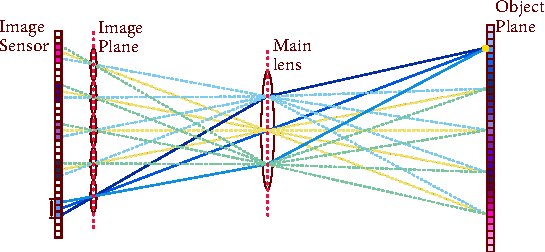
\includegraphics[width=0.6\textwidth]{Figures/Chapter2/photo_consistency.pdf}
    \caption[Light transformation model (focused on the plane).]{Light transformation model in a plenoptic camera. Within a plenoptic camera, a micro-lens array has been placed at the image plane, which further splits the incoming light rays from different directions and records them separately. Therefore, the multi-view information can be extracted from each light field image captured by a single shot.}
    \label{fig:photo_consistency_with_nickname}
\end{figure}
Following the Table of Contents, the template includes the lists of tables, figures and algorithms, abbreviations and symbols. The numbering, capitalisation and wording of the titles of every items listed agree exactly with the manner in which they appear in the body text. For the illustration with a long title, users can also provide a ``nickname'' of the illustration by enclosing the it in the square brackets. For example, \figref{fig:photo_consistency} and \figref{fig:photo_consistency_with_nickname} have the same image captions in the body text, but the wordings appear in the Table of Contents are different. \figref{fig:photo_consistency_with_nickname} uses the wordings in the square brackets as its caption, as shown at page \darkred{vii}.


%----------------------------------------------------------------------------------------
%	THESIS CONTENT - APPENDICES
%----------------------------------------------------------------------------------------

\appendix % Cue to tell LaTeX that the following "chapters" are Appendices

% Include the appendices of the thesis as separate files from the Appendices folder
% Uncomment the lines as you write the Appendices

% Appendix A

\chapter{About Appendix} % Main appendix title
\label{AppendixA} % For referencing this appendix elsewhere, use \ref{AppendixA}
The appendix is usually used to provide some supplementary materials for the publications. For example, some experimental results, network architecture, detailed experimental settings or proving of the theories. You can have more than one appendices to provide the materials for different uses.

% Appendix Template

\chapter{Appendix Title Here} % Main appendix title

\label{AppendixX} % Change X to a consecutive letter; for referencing this appendix elsewhere, use \ref{AppendixX}

Write your Appendix content here.
% Appendix Template

\chapter{Appendix Title Here} % Main appendix title

\label{AppendixX} % Change X to a consecutive letter; for referencing this appendix elsewhere, use \ref{AppendixX}

Write your Appendix content here.


%----------------------------------------------------------------------------------------
%	BIBLIOGRAPHY
%----------------------------------------------------------------------------------------

\printbibliography[heading=bibintoc]

%----------------------------------------------------------------------------------------

\end{document}
